%\setcounter{chapter}{2}

%    https://tex.stackexchange.com/questions/40725/how-to-change-the-font-size-during-the-new-defined-environment
%    http://www.sascha-frank.com/latex-font-size.html
%\begin{normalsize}
\begin{small}
%\begin{footnotesize}


\chapter{Physics Object Reconstruction}
\label{ch:cms_reco}

Excellent spatial resolution of the CMS trackers, high granularity of the calorimeters, and almost $4\pi$ coverage of the detector, allowed the CMS to introduce the particle flow (PF) algorithm \cite{Particle_flow} for a global event reconstruction. PF takes the input from all subdetectors, analyses the redundant information, removes the duplicate one, and forms the physics objects. PF procedure starts with identification of tracks and calorimeter clusters, then the reconstruction of the physics objects is performed, such as electrons, muons, jets, etc. In this section we will discuss the whole PF approach and all key elements of this reconstruction sequence.
  
  
\section{Track Reconstruction}\label{sec:track_reconstruction}

The reconstruction starts with the clusters of signals (``hits'') in the inner tracker. The information from these clusters in the Pixel and Strip subdetectors is aggregated based on their signal-to-noise ratios. The charge-weighted averaging is performed (for different particle charge hypothesis), as well as other corrections are further applied to identify the real hit positions. 

The helix trajectory that the particle follows in the magnetic field inside of the detector is characterised by five parameters: the direction in $\eta$, the 3D position with respect to the reference point, which is the centre of the IP, and the curvature of the track with the radius R. This information is enough to compute estimates of basic physics quantities, however, the this task is complicated by the presence of event high multiplicity (number of charged particles produced in the same event) and also by the physics aspect of the electron propagation in matter: an electron traversing the detector has nearly 85 $\%$ probability to emit a bremsstrahlung photon. Hadronic effects also need to be taken into account: a hadron has a 20 $\%$ probability to experience multiple scattering on the nuclei of the detector before reaching the HCAL. 

To keep the track finding efficiency high, while maintaining low the efficiency of miss-identified tracks, track reconstruction is performed sequentially using the combinatorial track finder (CTF) \cite{combined_track_finding}. First the "purest" tracks are reconstructed, they have high $p_T$ and the hits point towards the primary vertex (PV). The term PV is used to refer to the vertex which is the actual point of origin of the produced particle, when several other hard scattering vertices are present in the event. Then these pure tracks are removed from the collection of tracks and another round of the track reconstruction starts. This procedure applied several times reduces the combinatorial factor and also simplifies the identification of tracks with the low $p_T$ or those which do not point to the PV. During each iteration, the reconstruction follows these steps:

\begin{itemize}
\item Seed generation. Rough estimates of the particle trajectories ("seeds") are produced using either three hits or two hits and a PV constraint. Based on which iteration the algorithm is at, some additional constraints are applied, e.g., a minimal $p_T$ requirement, the need for the seed to originate close to the beam spot, etc. 
\item Trajectory building. Initial seeds are projected towards the compatible hits in the next layers based on the Kalman Filter (KF) procedure \cite{Kalman_filter}. The extrapolation is done until the outermost layer of the tracker is reached or when a "terminating condition" is satisfied, e.g., when the iteration accumulated the maximum number of invalid hits ("fake hits"). Each obtained trajectory is updated using a KF approach based on the compatibility of hits to form a better track candidate. The procedure is complicated by the fact that the same initial seed can give rise to several track candidates or vice versa, the same track candidate may be compatible with different seeds. Additionally, the trajectory building step should take into account energy loses of the particle due to multiple scattering on the detector material, inhomogeneities of the tracker material, and the effects of the regions of non constant magnetic field. 
\item Track fitting. After the track candidate has been built, the track parameters are refitted by a KF and the "smoother". This step uses the full available information about the track and gives optimal estimates of the track parameters. To remove a large number of fake tracks, which are present due to a very complicated nature of the problem and the high track multiplicity in the event, a multivariate (MVA) selection is applied. MVA incorporates variables that discriminate real tracks from the fakes: the signed transverse curvature and impact parameters (with respect to the beam spot), the polar and azimuthal angles, number of missing hits, the fit quality variables, etc. 
\end{itemize}

The CTF procedure runs for 10 iterations. For 2016 collisions with a mean pileup (additional hard scattering vertices) of 24, the CTF efficiency to identify real tracks varied from 80 to 95$\%$ with the mis-identification efficiency of 5 - 10 $\%$.



\subsection{Muon tracking}\label{sec:muon_track_reconstruction}

Muons are detected by the inner tracker and also by the outer (muon) tracker. This greatly improves muon track reconstruction and motivated the development of a dedicated muon reconstruction algorithms. The ninth and the tenth iterations of the CTF are focused on the muon reconstruction. These iterations are using three separate algorithms to identify: 

\begin{itemize}

\item Standalone muons. This algorithms uses only muon tracker information: DTs, CSCs, RPCs. Hits from the inner chambers are used as seeds and projected to hits in the outer chambers. Then, a standard KF procedure is used to identify track candidates, which are called standalone muons.
\item Tracker muons. Only the inner tracking information is used to form tracks. Tracks are further projected to muon subsystems, where a compatibility with at least one muon hit is required. This algorithm works with low momentum muons: tracks with $p_T$ above 0.5 GeV and a total momentum greater than 2.5 GeV.
\item Global muons. Tracker tracks and standalone tracks are projected to the outermost layer of the muon system, checking the compatibility between two approaches. The resulting combined set of track hits is refitted to produce a global muon track. Mostly high momentum muons with $p_T > $ ?? 200 GeV profit from this algorithm.
\end{itemize}


\subsection{Electron tracking}\label{sec:ele_track_reconstruction}
Electrons are also detected by the inner tracker, however, their reconstruction is complicated by the fact that they emit bremsstrahlung photons and the trajectory becomes more complex. As a result, the clustering algorithms need also to identify the bremsstrahlung photons and account for the fact that the energy clusters corresponding to these photons may be located outside of the main electron trajectory, when extrapolated to the ECAL. 

Since a KF approach assumes that energy losses are Gaussian, and this is not the case for electrons, a dedicated procedure is developed - a modified KF - the Gaussian Sum Filter (GSF) \cite{GSF}. In this method the radiated energy losses are approximated by the sum of Gaussian distributions. 

The electron seeds for the GSF are built using the ECAL information. Two different approaches are developed for the track reconstruction:

\begin{itemize}

\item Super Cluster based electrons. Cluster of energy in the ECAL and grouped together to form super clusters (SCs). Using the information of the energy spread among the clusters, the curvature of the electrons is estimated and tracker seeds are formed, with the SC position as a constraint. 
\item Tracks based electrons. Tracks from the inner tracker are projected to ECAL clusters, checking the compatibility using quality variables, such as $\chi^2$, number of missing hits (absent hits along the path of the track), etc. 
\end{itemize}

A typical momentum resolution for electrons in $Z \rightarrow e^- e^+$ decays is approximately 1.7 - 4.5$\%$.

\subsection{Primary Vertex reconstruction}\label{sec:PV_reconstruction}

At the LHC energies, several hard scattering vertices are produced in each collision. The location of all primary vertices (PV) is reconstructed using the tracks. However, normally only one (the main PV) out of these vertices (referred to as additional vertices or pileup) produces the interesting physics interactions. All the vertices are important since they are reused in the feed-back loop of the track reconstruction procedure. Also, a precise identification of primary vertices is important for determining the effect of the pileup on all physics objects in general and b-tagging in particular (will be discussed later in this chapter). 



The PV identification consists of three steps: the tracks are selected, then the tracks from the same PV are combined in clusters, and, finally, the position of the PV is determined from the fits to tracks.

Selecting the tracks, only those consistent with the location of the PV are considered. Several variables are used to improve the quality of the track selection procedure: the transverse impact parameter (the relative distance in the vertical plane with respect to the centre of the beam spot),  the number of strip and pixel hits associated with a track, and the $\chi^2$ of the fit .

Clustering of the tracks is based on their z position with respect to the beam spot. A deterministic annealing (DA) algorithm \cite{DeterministicAnnealing} is used to find the global minimum for this problem with many degrees of freedom. The idea of this algorithm is based on the physics example of a system approaching a state of minimal energy through a series of temperature  reductions. 

Once the clustering is completed and PVs are identified, the candidates with more than two tracks are fitted using an adaptive vertex fitter \cite{AdaptiveVertexFitting}. The result of this procedure is a set of probabilities assigned to tracks. This can be thought of as a likelihood that the track originated from the given vertex.


The resolution of PVs varies between 10 - 100 $\mu$m to 100 ?m and depends on track qualities. The main PV is determined as the vertex with the highest sum of the squared $p_T$.


\subsection{Particle Flow links and blocks}\label{sec:some_reconstruction}

Usually a particle leaves the signal in several CMS dubdetectors which is stored as PF \cite{ParticleFlow} elements. To connect these PF elements, the link algorithm (LA) was developed. The LA can test any pair of elements in the event. To speed up the calculations, only pairs of elements that are "neighbours" in the specified $\eta - \varphi$ plane are considered. When the pair of elements is linked, the LA determines the distance between the elements which is related to the quality of the link. This procedure produces PF blocks of elements, which are linked either by a direct, or an indirect link (through the common elements)


%%%%%%%%%%%%%%%%%%%%%%%%%%%%
  
  - somewhere a section on physics objects where you discuss that there are tracks, there are jets, there are b-jets, what it means an isolated lepton, what it means missing momentum, and so forth. For example, Ekaterina has a section on particle flow, if I remember right, where she discusses that. Or you can have a section that just discuses the proton-proton collisions environment and explains that many particles created in collisions are unstable and decay right away. What is observable in an experiment such as CMS is longer-lived or stable particles. These include electrons, muons, photons, and some ground state hadrons. At the same time, energetic quarks or gluons hadronize and can be seen in a particle detectors as jets of hadrons (so define jets here). Same for tau leptons, we detect them either as electrons/muons, or hadronic jets. Etc. If you have such a conceptual paragraph here, some time later you can have a particle flow discussion when it is time to be more specific. But discussion at this level above would allow you to then discuss the requirements on CMS design using terms like b-jets or isolated leptons.




\begin{figure}[H]
  \centering
  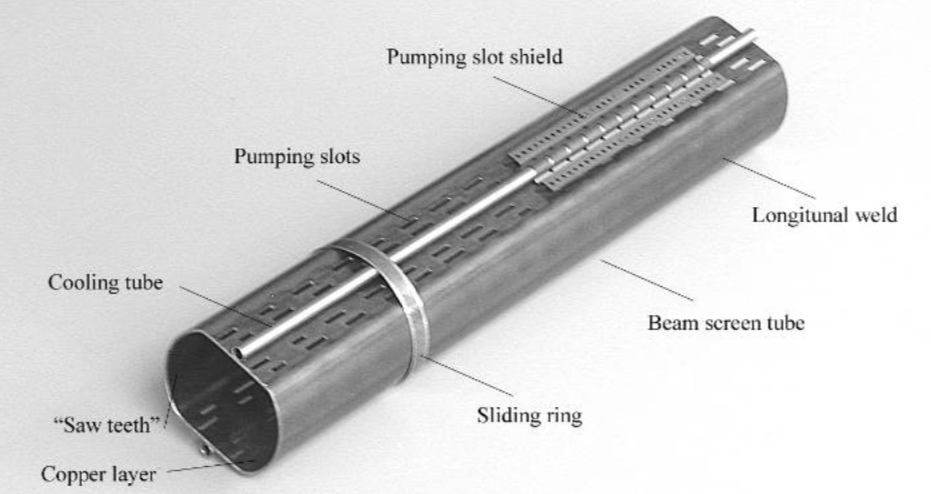
\includegraphics[width=0.7\textwidth]{beam_screen}
  \caption{Beam screen.}\label{beam_screen}
\end{figure}






  EGAMMA AT LEAST SAY THAT HAS BEEN WORKING AND SHOW SOME PLOTS?



%\end{normalsize}       % 28 to 58 -> 31 pages for the chapter (font 12)
\end{small}             % 28 to 56 -> 29 pages for the chapter (font almost 11)
%\end{footnotesize}  % 28 to 51 -> 24 pages for the chapter (font 10)
 
